% -*- mode: latex; -*-
\DocumentMetadata{pdfstandard=X-4p}
\documentclass[aspectratio=169,8pt]{beamer}
\usetheme{metropolis}

% Standard packages

\usepackage[english]{babel}
%\usepackage[latin1]{inputenc}
%\usepackage{times}
%\usepackage[T1]{fontenc}
\usepackage{fontspec}
\usepackage[]{unicode-math}
\setsansfont{Roboto}
\usepackage{amsmath}

% Setup asymptote
\usepackage[inline]{asymptote}

\newcounter{counter}
% Author, Title, etc.

\title{Heaps}

\author[Shiv Shankar Dayashru]{Shiv Shankar Dayashru}

\begin{document}
\begin{frame}
  \titlepage
\end{frame}
\begin{frame}{Heaps}
  There are two different types of heaps. Min-heap and max-heap. A heap is a complete binary tree that
  satisfies the heap property i.e. for every node, the value of its children is less(max-heap or more for
  min-heap) than or equal to its own value. Heaps are often used to implement priority queues, where the
  smallest or the largest element is always at the top.
  \begin{center}
    \begin{figure}
      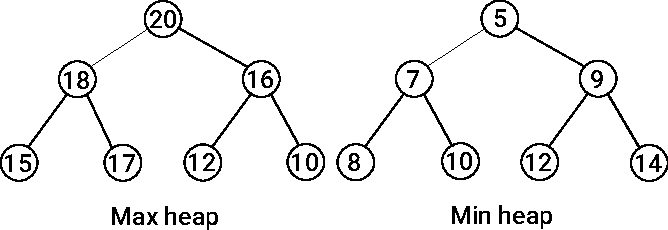
\includegraphics{heap1}
    \end{figure}
  \end{center}
\end{frame}
\begin{frame}{Properties of a Heap}
  \begin{itemize}
  \item A heap is a complete binary tree. This implies that all levels are fully filled except last level
    i.e. leaf nodes exist only at the last level.
  \item The largest or the smallest value is always at the top.
  \item Parent and child have a special relationship. If index or parent is $i$ then children are at index
    $2i + 1$ and $2i + 2$ for $0$-based indexing.
  \item Insertion and removal are efficient and have a time complexity $O(\log n)$.
  \item Efficient access to the largest or smallest element with a time complexity of $O(1)$.
  \end{itemize}
\end{frame}
\begin{frame}{Insertion in Heaps}
  \begin{center}
    \begin{figure}
      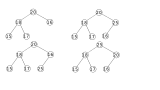
\includegraphics{heap2}
    \end{figure}
  \end{center}
\end{frame}
\begin{frame}{Deletion in Heaps}
  \begin{center}
    \begin{figure}
      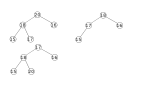
\includegraphics{heap3}
    \end{figure}
  \end{center}
\end{frame}
\end{document}